\section{ТЕСТИРОВАНИЕ РАЗРАБОТАННОГО МОДУЛЯ ДИСЦИПЛИНЫ ОБСЛУЖИВАНИЯ CLASS-BASED WFQ}

	\subsection{Описание тестовой среды}

		Для тестирования модуля ядра была создана система виртуальных машин на основе
		системы эмуляции программного обеспечения QEMU. Схема тестовой среды представлена
		на Рисунке~\ref{pic:testscheme}. Источником служит узел, от которого исходит трафик;
		таблицы маршрутизации настроены таким образом, чтобы весь трафик, который
		должен попасть на узел-цель шёл через промежуточный узел, на котором
		настроена тестируемая дисциплина обслуживания CBWFQ.

        \begin{figure}[ht!]
        	\center
        	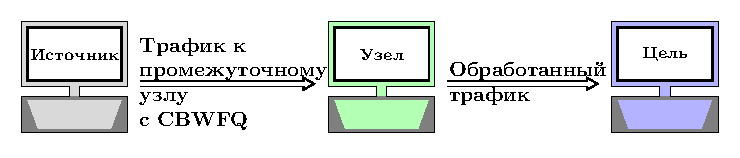
\includegraphics[scale=1.2]{pdfimages/test_scheme.pdf}
        	\caption{Схема тестовой среды.}
			\label{pic:testscheme}
        \end{figure}

		В Листинге~\ref{lst:tccmd} приведена система настройки дисциплины на промежуточном узле.
        \begin{figure}[ht!]
    		\center
    		\begin{lstlisting}[frame=lines,
    						  caption={Список команд для конфигурации дисциплины обслуживания CBWFQ.},
    						  label={lst:tccmd},
    						  style=tcstyle]
tc qdisc add dev $IFACE root handle 1: cbwfq bandwidth \
		100Mbps default rate 5Mbps
tc class add dev $IFACE parent 1: classid 1:2 cbwfq \
		 rate 25Mbps
tc class add dev $IFACE parent 1: classid 1:3 cbwfq \
		 rate 70Mbps
tc filter add dev ens4 parent 1:1 protocol ip u32 match \
        ip dport $TESTPORT1 0xffff flowid 1:2
tc filter add dev ens4 parent 1:0 protocol ip u32 match \
        ip dport $TESTPORT2 0xffff flowid 1:3
    		\end{lstlisting}
        \end{figure}
%$
		Переменные окружения \lstinline{TESTPORT1} и \lstinline{TESTPORT2} содержат в себе номера портов,
		с которых будет отправлен трафик на сервер. При добавлении дисциплины
		на интерфейс необходимо указать пропускную способность канала и выделенную
		пропускную способность для класса по умолчанию; размер
		очереди по умолчанию назначается опционально. При конфигурации классов
		в третьей и пятой строках происходит назначения пропускной способности для класса
		(возможно также назначение полосы в процентах от общей пропускной способности).
        В седьмой и девятой строках происходит
		назначение фильтров, которые будут направлять трафик с исходнымым портами \lstinline{TESTPORT1}
		и \lstinline{TESTPORT2}
		в очередь класса 1:2 и 1:3 соответственно. На один класс можно назначит множество фильтров
		(Linux предоставляет гибкие возможности по настройке фильтрации); это не
		контролируется непосредственно дисциплиной и находится в компетенции
		пользователя. 

		\subsection{Анализ точности выделения канала при конкурирующем трафике}
			
			Первый эксперимент заключается в исследовании разделения канала между
			двумя потоками трафика, приходящими со скоростью, больше скорости канала на
			промежуточном узле.

    		С использованием описанной конфигурации и указанных в Листингах~\ref{lst:iperfsrc} и~\ref{lst:iperfdst}
			команд произвелось десять испытаний в рамках эксперимента (схема
			эксперимента представлена на Рисунке~\ref{pic:exp1}).

		\begin{figure}[ht!]
			\center
			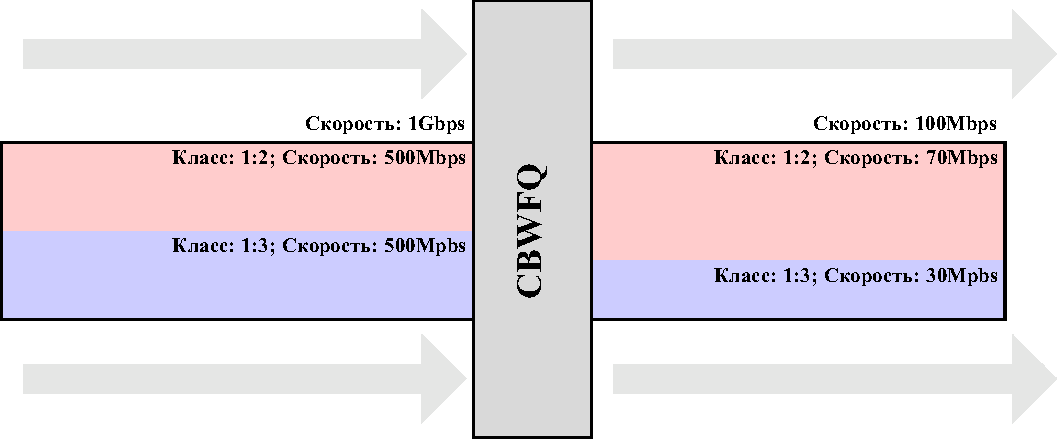
\includegraphics[scale=0.9]{./pdfimages/exp_scheme.pdf}
			\caption{Условная схема эксперимента 1.}
			\label{pic:exp1}
		\end{figure}

        \begin{figure}[ht!]
    		\center
    		\begin{lstlisting}[frame=lines,
    						  caption={Команда iperf на узле-источнике (клиентская сторона).},
    						  label={lst:iperfsrc}]
iperf3 -c $SERVERIP -p $TESRPORT1 -b 500M -u -t 90
iperf3 -c $SERVERIP -p $TESRPORT2 -b 500M -u -t 90
    		\end{lstlisting}
        \end{figure}	
        \begin{figure}[ht!]
    		\center
    		\begin{lstlisting}[frame=lines,
    						  caption={Команда iperf на узле-цели (серверная сторона).},
    						  label={lst:iperfdst}]
iperf3 -s -p $TESTPOR1 --logfile class2"$EXPNUM".log
iperf3 -s -p $TESTPOR2 --logfile class3"$EXPNUM".log
    		\end{lstlisting}
        \end{figure}


    		В течение экспериментов собирались отчёты от утилиты iperf со стороны сервера в
    		течение 90-та секунд. Отчёты представляют собой таблицу с полями:
			временной интервал (в секундах), количество переданных данных и пропускная способность.
			На каждый временной интервал таблица содержит описанную информацию для двух потоков.

			Результаты эксперимента можно наблюдать на Рисунке~\ref{pic:plot}.



            \begin{figure}[ht!]
            	\center
            	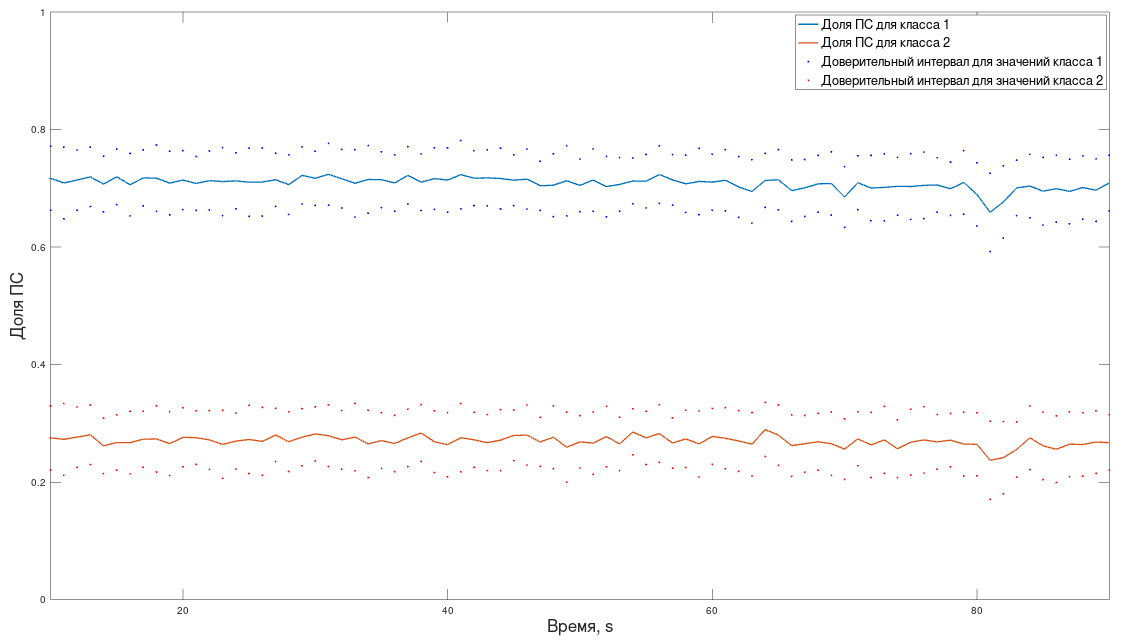
\includegraphics[width=0.9\linewidth]{./plotc.png} %{pdfimages/plots/plot_comet.pdf}
            	\caption{График распределения доли пропускной способности (ПС) по типам трафика в течение времени.
						 Среднее значение процента ПС для класса 1: $71 \pm 3 \%$ $(P = 0.95)$.
                         Среднее значение процента ПС для класса 2: $27 \pm 2 \%$ $(P = 0.95)$.
                        }
    			\label{pic:plot}
            \end{figure}

			Доля пропускной
			способности для первого и второго класса соответствует минимальной сконфигурированной доле, выделенной
			этим классам (или их весу $\dfrac{\text{70Mbps}}{\text{100Mbps}} = 0.7$ и
            $\dfrac{\text{25Mbps}}{\text{100Mbps}} = 0.25$ соответственно).
			Эти доли означают минимальное количество, выделяемое классу. В данном
			эксперименте классы получили пропускную способность больше сконфигурированной
			из-за того, что часть неутилизированной пропускной способности класса по умолчанию
			распределилась между ними.

		%\newpage
		\subsection{Анализ точности выделения канала при независимом трафике}

			Второй эксперимент заключается в исследовании разделения канала между
			двумя потоками трафика, приходящими со скоростью, суммарно меньше
			скорости канала и соответствующие конфигурационным параметрам.

    		С использованием описанной конфигурации и указанных в Листингах~\ref{lst:iperfsrc2} и~\ref{lst:iperfdst2}
			команд произвелось десять испытаний в рамках эксперимента (схема

	        \begin{figure}[ht!]
    		\center
    		\begin{lstlisting}[frame=lines,
    						  caption={Команда iperf на узле-источнике (клиентская сторона).},
    						  label={lst:iperfsrc2}]
iperf3 -c $SERVERIP -p $TESRPORT1 -b 100M -u -t 90
iperf3 -c $SERVERIP -p $TESRPORT2 -b 5M -u -t 90
    		\end{lstlisting}
        \end{figure}	
%$
        \begin{figure}[ht!]
    		\center
    		\begin{lstlisting}[frame=lines,
    						  caption={Команда iperf на узле-цели (серверная сторона).},
    						  label={lst:iperfdst2}]
iperf3 -s -p $TESTPOR1 --logfile class2"$EXPNUM".log
iperf3 -s -p $TESTPOR2 --logfile class3"$EXPNUM".log
    		\end{lstlisting}
%$		эксперимента представлена на Рисунке~\ref{pic:exp2}).
        \end{figure}

		\begin{figure}[ht!]
			\center
			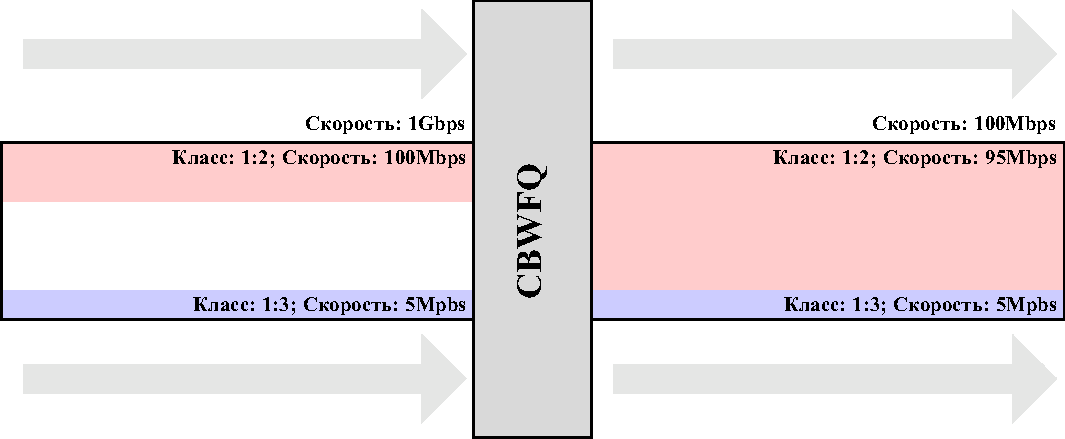
\includegraphics[scale=0.9]{./pdfimages/exp_scheme2.pdf}
			\caption{Условная схема эксперимента 2.}
			\label{pic:exp2}
		\end{figure}

    		В течение экспериментов собирались отчёты от утилиты iperf со стороны сервера в
    		течение 90-та секунд. Отчёты имеют тот же формат, что и описанный в прошлом эксперименте.

			Результаты эксперимента можно наблюдать на Рисунке~\ref{pic:plot2}.


            \begin{figure}[ht!]
            	\center
            	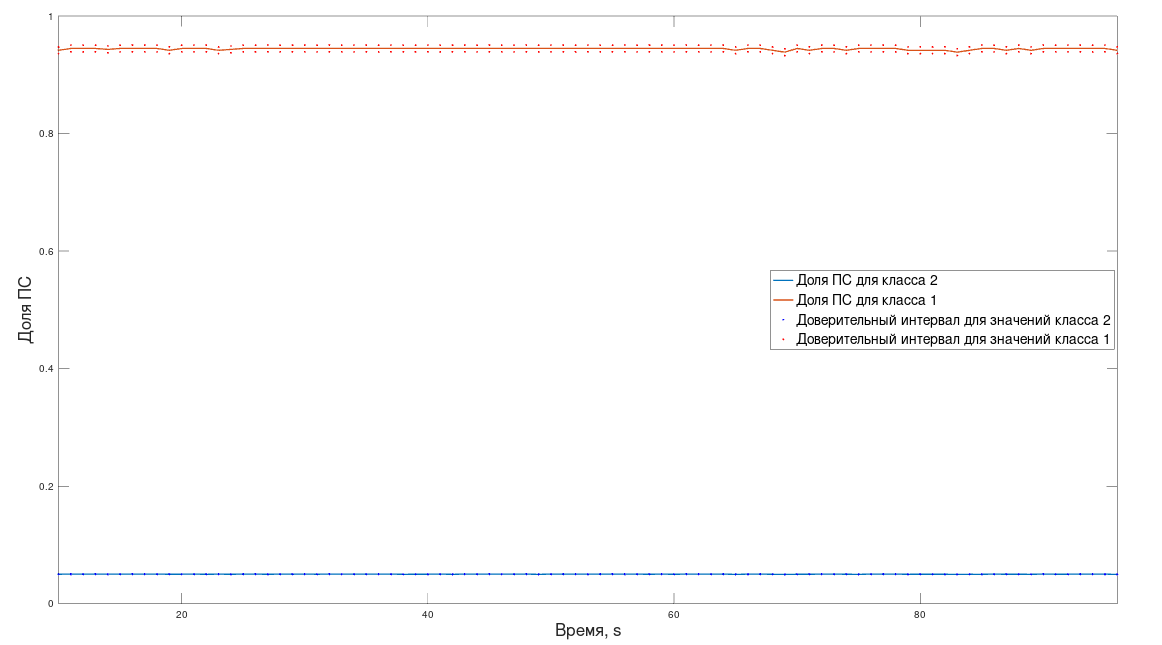
\includegraphics[width=\linewidth]{./plotnc.png} %{pdfimages/plots/plot_no_compet.pdf}
            	\caption{График распределения доли пропускной способности (ПС) по типам трафика в течение времени.
						 Среднее значение процента  ПС для класса 1: $94 \pm 0.5 \%$ $(P = 0.95)$.
                         Среднее значение процента  ПС для класса 2: $5 \pm 0.07 \%$ $(P = 0.95)$}
    			\label{pic:plot2}
            \end{figure}

			В данном
			случае второй класс получает всю требуемую ему пропускную способность; в этом
			факте и состоит отсутствие конкуренции: второй поток не пытается занять больше,
			чем ему назначенно. Поток первого класса занимает оставшуюся свободную часть канала.
			
